
% Default to the notebook output style

    


% Inherit from the specified cell style.




    
\documentclass[11pt]{article}

    
    
    \usepackage[T1]{fontenc}
    % Nicer default font (+ math font) than Computer Modern for most use cases
    \usepackage{mathpazo}

    % Basic figure setup, for now with no caption control since it's done
    % automatically by Pandoc (which extracts ![](path) syntax from Markdown).
    \usepackage{graphicx}
    % We will generate all images so they have a width \maxwidth. This means
    % that they will get their normal width if they fit onto the page, but
    % are scaled down if they would overflow the margins.
    \makeatletter
    \def\maxwidth{\ifdim\Gin@nat@width>\linewidth\linewidth
    \else\Gin@nat@width\fi}
    \makeatother
    \let\Oldincludegraphics\includegraphics
    % Set max figure width to be 80% of text width, for now hardcoded.
    \renewcommand{\includegraphics}[1]{\Oldincludegraphics[width=.8\maxwidth]{#1}}
    % Ensure that by default, figures have no caption (until we provide a
    % proper Figure object with a Caption API and a way to capture that
    % in the conversion process - todo).
    \usepackage{caption}
    \DeclareCaptionLabelFormat{nolabel}{}
    \captionsetup{labelformat=nolabel}

    \usepackage{adjustbox} % Used to constrain images to a maximum size 
    \usepackage{xcolor} % Allow colors to be defined
    \usepackage{enumerate} % Needed for markdown enumerations to work
    \usepackage{geometry} % Used to adjust the document margins
    \usepackage{amsmath} % Equations
    \usepackage{amssymb} % Equations
    \usepackage{textcomp} % defines textquotesingle
    % Hack from http://tex.stackexchange.com/a/47451/13684:
    \AtBeginDocument{%
        \def\PYZsq{\textquotesingle}% Upright quotes in Pygmentized code
    }
    \usepackage{upquote} % Upright quotes for verbatim code
    \usepackage{eurosym} % defines \euro
    \usepackage[mathletters]{ucs} % Extended unicode (utf-8) support
    \usepackage[utf8x]{inputenc} % Allow utf-8 characters in the tex document
    \usepackage{fancyvrb} % verbatim replacement that allows latex
    \usepackage{grffile} % extends the file name processing of package graphics 
                         % to support a larger range 
    % The hyperref package gives us a pdf with properly built
    % internal navigation ('pdf bookmarks' for the table of contents,
    % internal cross-reference links, web links for URLs, etc.)
    \usepackage{hyperref}
    \usepackage{longtable} % longtable support required by pandoc >1.10
    \usepackage{booktabs}  % table support for pandoc > 1.12.2
    \usepackage[inline]{enumitem} % IRkernel/repr support (it uses the enumerate* environment)
    \usepackage[normalem]{ulem} % ulem is needed to support strikethroughs (\sout)
                                % normalem makes italics be italics, not underlines
    

    
    
    % Colors for the hyperref package
    \definecolor{urlcolor}{rgb}{0,.145,.698}
    \definecolor{linkcolor}{rgb}{.71,0.21,0.01}
    \definecolor{citecolor}{rgb}{.12,.54,.11}

    % ANSI colors
    \definecolor{ansi-black}{HTML}{3E424D}
    \definecolor{ansi-black-intense}{HTML}{282C36}
    \definecolor{ansi-red}{HTML}{E75C58}
    \definecolor{ansi-red-intense}{HTML}{B22B31}
    \definecolor{ansi-green}{HTML}{00A250}
    \definecolor{ansi-green-intense}{HTML}{007427}
    \definecolor{ansi-yellow}{HTML}{DDB62B}
    \definecolor{ansi-yellow-intense}{HTML}{B27D12}
    \definecolor{ansi-blue}{HTML}{208FFB}
    \definecolor{ansi-blue-intense}{HTML}{0065CA}
    \definecolor{ansi-magenta}{HTML}{D160C4}
    \definecolor{ansi-magenta-intense}{HTML}{A03196}
    \definecolor{ansi-cyan}{HTML}{60C6C8}
    \definecolor{ansi-cyan-intense}{HTML}{258F8F}
    \definecolor{ansi-white}{HTML}{C5C1B4}
    \definecolor{ansi-white-intense}{HTML}{A1A6B2}

    % commands and environments needed by pandoc snippets
    % extracted from the output of `pandoc -s`
    \providecommand{\tightlist}{%
      \setlength{\itemsep}{0pt}\setlength{\parskip}{0pt}}
    \DefineVerbatimEnvironment{Highlighting}{Verbatim}{commandchars=\\\{\}}
    % Add ',fontsize=\small' for more characters per line
    \newenvironment{Shaded}{}{}
    \newcommand{\KeywordTok}[1]{\textcolor[rgb]{0.00,0.44,0.13}{\textbf{{#1}}}}
    \newcommand{\DataTypeTok}[1]{\textcolor[rgb]{0.56,0.13,0.00}{{#1}}}
    \newcommand{\DecValTok}[1]{\textcolor[rgb]{0.25,0.63,0.44}{{#1}}}
    \newcommand{\BaseNTok}[1]{\textcolor[rgb]{0.25,0.63,0.44}{{#1}}}
    \newcommand{\FloatTok}[1]{\textcolor[rgb]{0.25,0.63,0.44}{{#1}}}
    \newcommand{\CharTok}[1]{\textcolor[rgb]{0.25,0.44,0.63}{{#1}}}
    \newcommand{\StringTok}[1]{\textcolor[rgb]{0.25,0.44,0.63}{{#1}}}
    \newcommand{\CommentTok}[1]{\textcolor[rgb]{0.38,0.63,0.69}{\textit{{#1}}}}
    \newcommand{\OtherTok}[1]{\textcolor[rgb]{0.00,0.44,0.13}{{#1}}}
    \newcommand{\AlertTok}[1]{\textcolor[rgb]{1.00,0.00,0.00}{\textbf{{#1}}}}
    \newcommand{\FunctionTok}[1]{\textcolor[rgb]{0.02,0.16,0.49}{{#1}}}
    \newcommand{\RegionMarkerTok}[1]{{#1}}
    \newcommand{\ErrorTok}[1]{\textcolor[rgb]{1.00,0.00,0.00}{\textbf{{#1}}}}
    \newcommand{\NormalTok}[1]{{#1}}
    
    % Additional commands for more recent versions of Pandoc
    \newcommand{\ConstantTok}[1]{\textcolor[rgb]{0.53,0.00,0.00}{{#1}}}
    \newcommand{\SpecialCharTok}[1]{\textcolor[rgb]{0.25,0.44,0.63}{{#1}}}
    \newcommand{\VerbatimStringTok}[1]{\textcolor[rgb]{0.25,0.44,0.63}{{#1}}}
    \newcommand{\SpecialStringTok}[1]{\textcolor[rgb]{0.73,0.40,0.53}{{#1}}}
    \newcommand{\ImportTok}[1]{{#1}}
    \newcommand{\DocumentationTok}[1]{\textcolor[rgb]{0.73,0.13,0.13}{\textit{{#1}}}}
    \newcommand{\AnnotationTok}[1]{\textcolor[rgb]{0.38,0.63,0.69}{\textbf{\textit{{#1}}}}}
    \newcommand{\CommentVarTok}[1]{\textcolor[rgb]{0.38,0.63,0.69}{\textbf{\textit{{#1}}}}}
    \newcommand{\VariableTok}[1]{\textcolor[rgb]{0.10,0.09,0.49}{{#1}}}
    \newcommand{\ControlFlowTok}[1]{\textcolor[rgb]{0.00,0.44,0.13}{\textbf{{#1}}}}
    \newcommand{\OperatorTok}[1]{\textcolor[rgb]{0.40,0.40,0.40}{{#1}}}
    \newcommand{\BuiltInTok}[1]{{#1}}
    \newcommand{\ExtensionTok}[1]{{#1}}
    \newcommand{\PreprocessorTok}[1]{\textcolor[rgb]{0.74,0.48,0.00}{{#1}}}
    \newcommand{\AttributeTok}[1]{\textcolor[rgb]{0.49,0.56,0.16}{{#1}}}
    \newcommand{\InformationTok}[1]{\textcolor[rgb]{0.38,0.63,0.69}{\textbf{\textit{{#1}}}}}
    \newcommand{\WarningTok}[1]{\textcolor[rgb]{0.38,0.63,0.69}{\textbf{\textit{{#1}}}}}
    
    
    % Define a nice break command that doesn't care if a line doesn't already
    % exist.
    \def\br{\hspace*{\fill} \\* }
    % Math Jax compatability definitions
    \def\gt{>}
    \def\lt{<}
    % Document parameters
    \title{Assignment1}
    
    
    

    % Pygments definitions
    
\makeatletter
\def\PY@reset{\let\PY@it=\relax \let\PY@bf=\relax%
    \let\PY@ul=\relax \let\PY@tc=\relax%
    \let\PY@bc=\relax \let\PY@ff=\relax}
\def\PY@tok#1{\csname PY@tok@#1\endcsname}
\def\PY@toks#1+{\ifx\relax#1\empty\else%
    \PY@tok{#1}\expandafter\PY@toks\fi}
\def\PY@do#1{\PY@bc{\PY@tc{\PY@ul{%
    \PY@it{\PY@bf{\PY@ff{#1}}}}}}}
\def\PY#1#2{\PY@reset\PY@toks#1+\relax+\PY@do{#2}}

\expandafter\def\csname PY@tok@w\endcsname{\def\PY@tc##1{\textcolor[rgb]{0.73,0.73,0.73}{##1}}}
\expandafter\def\csname PY@tok@c\endcsname{\let\PY@it=\textit\def\PY@tc##1{\textcolor[rgb]{0.25,0.50,0.50}{##1}}}
\expandafter\def\csname PY@tok@cp\endcsname{\def\PY@tc##1{\textcolor[rgb]{0.74,0.48,0.00}{##1}}}
\expandafter\def\csname PY@tok@k\endcsname{\let\PY@bf=\textbf\def\PY@tc##1{\textcolor[rgb]{0.00,0.50,0.00}{##1}}}
\expandafter\def\csname PY@tok@kp\endcsname{\def\PY@tc##1{\textcolor[rgb]{0.00,0.50,0.00}{##1}}}
\expandafter\def\csname PY@tok@kt\endcsname{\def\PY@tc##1{\textcolor[rgb]{0.69,0.00,0.25}{##1}}}
\expandafter\def\csname PY@tok@o\endcsname{\def\PY@tc##1{\textcolor[rgb]{0.40,0.40,0.40}{##1}}}
\expandafter\def\csname PY@tok@ow\endcsname{\let\PY@bf=\textbf\def\PY@tc##1{\textcolor[rgb]{0.67,0.13,1.00}{##1}}}
\expandafter\def\csname PY@tok@nb\endcsname{\def\PY@tc##1{\textcolor[rgb]{0.00,0.50,0.00}{##1}}}
\expandafter\def\csname PY@tok@nf\endcsname{\def\PY@tc##1{\textcolor[rgb]{0.00,0.00,1.00}{##1}}}
\expandafter\def\csname PY@tok@nc\endcsname{\let\PY@bf=\textbf\def\PY@tc##1{\textcolor[rgb]{0.00,0.00,1.00}{##1}}}
\expandafter\def\csname PY@tok@nn\endcsname{\let\PY@bf=\textbf\def\PY@tc##1{\textcolor[rgb]{0.00,0.00,1.00}{##1}}}
\expandafter\def\csname PY@tok@ne\endcsname{\let\PY@bf=\textbf\def\PY@tc##1{\textcolor[rgb]{0.82,0.25,0.23}{##1}}}
\expandafter\def\csname PY@tok@nv\endcsname{\def\PY@tc##1{\textcolor[rgb]{0.10,0.09,0.49}{##1}}}
\expandafter\def\csname PY@tok@no\endcsname{\def\PY@tc##1{\textcolor[rgb]{0.53,0.00,0.00}{##1}}}
\expandafter\def\csname PY@tok@nl\endcsname{\def\PY@tc##1{\textcolor[rgb]{0.63,0.63,0.00}{##1}}}
\expandafter\def\csname PY@tok@ni\endcsname{\let\PY@bf=\textbf\def\PY@tc##1{\textcolor[rgb]{0.60,0.60,0.60}{##1}}}
\expandafter\def\csname PY@tok@na\endcsname{\def\PY@tc##1{\textcolor[rgb]{0.49,0.56,0.16}{##1}}}
\expandafter\def\csname PY@tok@nt\endcsname{\let\PY@bf=\textbf\def\PY@tc##1{\textcolor[rgb]{0.00,0.50,0.00}{##1}}}
\expandafter\def\csname PY@tok@nd\endcsname{\def\PY@tc##1{\textcolor[rgb]{0.67,0.13,1.00}{##1}}}
\expandafter\def\csname PY@tok@s\endcsname{\def\PY@tc##1{\textcolor[rgb]{0.73,0.13,0.13}{##1}}}
\expandafter\def\csname PY@tok@sd\endcsname{\let\PY@it=\textit\def\PY@tc##1{\textcolor[rgb]{0.73,0.13,0.13}{##1}}}
\expandafter\def\csname PY@tok@si\endcsname{\let\PY@bf=\textbf\def\PY@tc##1{\textcolor[rgb]{0.73,0.40,0.53}{##1}}}
\expandafter\def\csname PY@tok@se\endcsname{\let\PY@bf=\textbf\def\PY@tc##1{\textcolor[rgb]{0.73,0.40,0.13}{##1}}}
\expandafter\def\csname PY@tok@sr\endcsname{\def\PY@tc##1{\textcolor[rgb]{0.73,0.40,0.53}{##1}}}
\expandafter\def\csname PY@tok@ss\endcsname{\def\PY@tc##1{\textcolor[rgb]{0.10,0.09,0.49}{##1}}}
\expandafter\def\csname PY@tok@sx\endcsname{\def\PY@tc##1{\textcolor[rgb]{0.00,0.50,0.00}{##1}}}
\expandafter\def\csname PY@tok@m\endcsname{\def\PY@tc##1{\textcolor[rgb]{0.40,0.40,0.40}{##1}}}
\expandafter\def\csname PY@tok@gh\endcsname{\let\PY@bf=\textbf\def\PY@tc##1{\textcolor[rgb]{0.00,0.00,0.50}{##1}}}
\expandafter\def\csname PY@tok@gu\endcsname{\let\PY@bf=\textbf\def\PY@tc##1{\textcolor[rgb]{0.50,0.00,0.50}{##1}}}
\expandafter\def\csname PY@tok@gd\endcsname{\def\PY@tc##1{\textcolor[rgb]{0.63,0.00,0.00}{##1}}}
\expandafter\def\csname PY@tok@gi\endcsname{\def\PY@tc##1{\textcolor[rgb]{0.00,0.63,0.00}{##1}}}
\expandafter\def\csname PY@tok@gr\endcsname{\def\PY@tc##1{\textcolor[rgb]{1.00,0.00,0.00}{##1}}}
\expandafter\def\csname PY@tok@ge\endcsname{\let\PY@it=\textit}
\expandafter\def\csname PY@tok@gs\endcsname{\let\PY@bf=\textbf}
\expandafter\def\csname PY@tok@gp\endcsname{\let\PY@bf=\textbf\def\PY@tc##1{\textcolor[rgb]{0.00,0.00,0.50}{##1}}}
\expandafter\def\csname PY@tok@go\endcsname{\def\PY@tc##1{\textcolor[rgb]{0.53,0.53,0.53}{##1}}}
\expandafter\def\csname PY@tok@gt\endcsname{\def\PY@tc##1{\textcolor[rgb]{0.00,0.27,0.87}{##1}}}
\expandafter\def\csname PY@tok@err\endcsname{\def\PY@bc##1{\setlength{\fboxsep}{0pt}\fcolorbox[rgb]{1.00,0.00,0.00}{1,1,1}{\strut ##1}}}
\expandafter\def\csname PY@tok@kc\endcsname{\let\PY@bf=\textbf\def\PY@tc##1{\textcolor[rgb]{0.00,0.50,0.00}{##1}}}
\expandafter\def\csname PY@tok@kd\endcsname{\let\PY@bf=\textbf\def\PY@tc##1{\textcolor[rgb]{0.00,0.50,0.00}{##1}}}
\expandafter\def\csname PY@tok@kn\endcsname{\let\PY@bf=\textbf\def\PY@tc##1{\textcolor[rgb]{0.00,0.50,0.00}{##1}}}
\expandafter\def\csname PY@tok@kr\endcsname{\let\PY@bf=\textbf\def\PY@tc##1{\textcolor[rgb]{0.00,0.50,0.00}{##1}}}
\expandafter\def\csname PY@tok@bp\endcsname{\def\PY@tc##1{\textcolor[rgb]{0.00,0.50,0.00}{##1}}}
\expandafter\def\csname PY@tok@fm\endcsname{\def\PY@tc##1{\textcolor[rgb]{0.00,0.00,1.00}{##1}}}
\expandafter\def\csname PY@tok@vc\endcsname{\def\PY@tc##1{\textcolor[rgb]{0.10,0.09,0.49}{##1}}}
\expandafter\def\csname PY@tok@vg\endcsname{\def\PY@tc##1{\textcolor[rgb]{0.10,0.09,0.49}{##1}}}
\expandafter\def\csname PY@tok@vi\endcsname{\def\PY@tc##1{\textcolor[rgb]{0.10,0.09,0.49}{##1}}}
\expandafter\def\csname PY@tok@vm\endcsname{\def\PY@tc##1{\textcolor[rgb]{0.10,0.09,0.49}{##1}}}
\expandafter\def\csname PY@tok@sa\endcsname{\def\PY@tc##1{\textcolor[rgb]{0.73,0.13,0.13}{##1}}}
\expandafter\def\csname PY@tok@sb\endcsname{\def\PY@tc##1{\textcolor[rgb]{0.73,0.13,0.13}{##1}}}
\expandafter\def\csname PY@tok@sc\endcsname{\def\PY@tc##1{\textcolor[rgb]{0.73,0.13,0.13}{##1}}}
\expandafter\def\csname PY@tok@dl\endcsname{\def\PY@tc##1{\textcolor[rgb]{0.73,0.13,0.13}{##1}}}
\expandafter\def\csname PY@tok@s2\endcsname{\def\PY@tc##1{\textcolor[rgb]{0.73,0.13,0.13}{##1}}}
\expandafter\def\csname PY@tok@sh\endcsname{\def\PY@tc##1{\textcolor[rgb]{0.73,0.13,0.13}{##1}}}
\expandafter\def\csname PY@tok@s1\endcsname{\def\PY@tc##1{\textcolor[rgb]{0.73,0.13,0.13}{##1}}}
\expandafter\def\csname PY@tok@mb\endcsname{\def\PY@tc##1{\textcolor[rgb]{0.40,0.40,0.40}{##1}}}
\expandafter\def\csname PY@tok@mf\endcsname{\def\PY@tc##1{\textcolor[rgb]{0.40,0.40,0.40}{##1}}}
\expandafter\def\csname PY@tok@mh\endcsname{\def\PY@tc##1{\textcolor[rgb]{0.40,0.40,0.40}{##1}}}
\expandafter\def\csname PY@tok@mi\endcsname{\def\PY@tc##1{\textcolor[rgb]{0.40,0.40,0.40}{##1}}}
\expandafter\def\csname PY@tok@il\endcsname{\def\PY@tc##1{\textcolor[rgb]{0.40,0.40,0.40}{##1}}}
\expandafter\def\csname PY@tok@mo\endcsname{\def\PY@tc##1{\textcolor[rgb]{0.40,0.40,0.40}{##1}}}
\expandafter\def\csname PY@tok@ch\endcsname{\let\PY@it=\textit\def\PY@tc##1{\textcolor[rgb]{0.25,0.50,0.50}{##1}}}
\expandafter\def\csname PY@tok@cm\endcsname{\let\PY@it=\textit\def\PY@tc##1{\textcolor[rgb]{0.25,0.50,0.50}{##1}}}
\expandafter\def\csname PY@tok@cpf\endcsname{\let\PY@it=\textit\def\PY@tc##1{\textcolor[rgb]{0.25,0.50,0.50}{##1}}}
\expandafter\def\csname PY@tok@c1\endcsname{\let\PY@it=\textit\def\PY@tc##1{\textcolor[rgb]{0.25,0.50,0.50}{##1}}}
\expandafter\def\csname PY@tok@cs\endcsname{\let\PY@it=\textit\def\PY@tc##1{\textcolor[rgb]{0.25,0.50,0.50}{##1}}}

\def\PYZbs{\char`\\}
\def\PYZus{\char`\_}
\def\PYZob{\char`\{}
\def\PYZcb{\char`\}}
\def\PYZca{\char`\^}
\def\PYZam{\char`\&}
\def\PYZlt{\char`\<}
\def\PYZgt{\char`\>}
\def\PYZsh{\char`\#}
\def\PYZpc{\char`\%}
\def\PYZdl{\char`\$}
\def\PYZhy{\char`\-}
\def\PYZsq{\char`\'}
\def\PYZdq{\char`\"}
\def\PYZti{\char`\~}
% for compatibility with earlier versions
\def\PYZat{@}
\def\PYZlb{[}
\def\PYZrb{]}
\makeatother


    % Exact colors from NB
    \definecolor{incolor}{rgb}{0.0, 0.0, 0.5}
    \definecolor{outcolor}{rgb}{0.545, 0.0, 0.0}



    
    % Prevent overflowing lines due to hard-to-break entities
    \sloppy 
    % Setup hyperref package
    \hypersetup{
      breaklinks=true,  % so long urls are correctly broken across lines
      colorlinks=true,
      urlcolor=urlcolor,
      linkcolor=linkcolor,
      citecolor=citecolor,
      }
    % Slightly bigger margins than the latex defaults
    
    \geometry{verbose,tmargin=1in,bmargin=1in,lmargin=1in,rmargin=1in}
    
    

    \begin{document}
    
    
    \maketitle
    
    

    
    \begin{Verbatim}[commandchars=\\\{\}]
{\color{incolor}In [{\color{incolor}1}]:} \PY{k+kn}{from} \PY{n+nn}{helper} \PY{k}{import} \PY{o}{*}
\end{Verbatim}


    Click
\href{https://github.com/Hammania689/prob_n_stats_II/blob/master/chp6/helper.py}{here}
to view contents of helper

    \begin{figure}
\centering
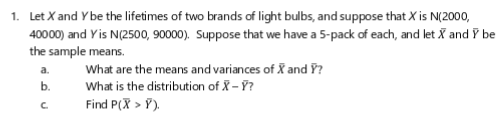
\includegraphics{images/num1.png}
\caption{alt text}
\end{figure}

    \hypertarget{a-what-are-the-means-and-variances-of-barx-and-bary}{%
\subsection{\texorpdfstring{A) What are the means and variances of
\(\bar{X}\) and
\(\bar{Y}\)?}{A) What are the means and variances of \textbackslash{}bar\{X\} and \textbackslash{}bar\{Y\}?}}\label{a-what-are-the-means-and-variances-of-barx-and-bary}}

\(\mu_\bar{X} = 2000\) \({\sigma_\bar{X}}^2 = 40000\)

\(\mu_\bar{Y} = 2500\) \({\sigma_\bar{Y}}^2 = 90000\)

    \hypertarget{b-what-is-the-distribution-of-barx---bary}{%
\subsection{\texorpdfstring{B) What is the distribution of \(\bar{X}\) -
\(\bar{Y}\)?}{B) What is the distribution of \textbackslash{}bar\{X\} - \textbackslash{}bar\{Y\}?}}\label{b-what-is-the-distribution-of-barx---bary}}

\(\bar{X} - \bar{Y} \approx\)

\$N(\mu\emph{\bar\{X\} - \mu}\bar\{Y\}, \{\sigma\emph{\bar\{X\}\}\^{}2 +
\{\sigma}\bar\{Y\}\}\^{}2 ) \approx \$

\(N(2000 - 2500, 40000 + 90000) \approx\) \#\# \$N(-500, 130000) \$

    \hypertarget{c-find-pbarx-bary}{%
\subsection{\texorpdfstring{C) Find
\(P(\bar{X} > \bar{Y})\)}{C) Find P(\textbackslash{}bar\{X\} \textgreater{} \textbackslash{}bar\{Y\})}}\label{c-find-pbarx-bary}}

\$P(\bar\{X\} \textgreater{} \bar\{Y\}) \approx P(\bar\{X\} - \bar\{Y\}
\textgreater{} 0) \approx \$

\hypertarget{keeping-part-b-in-mind}{%
\subsubsection{\texorpdfstring{\emph{Keeping part B in
mind\ldots{}}}{Keeping part B in mind\ldots{}}}\label{keeping-part-b-in-mind}}

\$N(\mu\emph{\bar\{X\} - \mu}\bar\{Y\}, \{\sigma\emph{\bar\{X\}\}\^{}2 +
\{\sigma}\bar\{Y\}\}\^{}2 ) \approx N(-500, 130000) \$

\$ P( \frac{\bar{X} - \bar{Y} }{\sqrt{130000}} \textgreater{}
\frac{0 -                     ( -500)}{\sqrt{130000}}) \approx P(Z
\textgreater{} 1.3867504905630728) \approx \$

\hypertarget{pz-1.39-approx-.0823}{%
\subsection{\texorpdfstring{\(P(Z > 1.39) \approx .0823\)}{P(Z \textgreater{} 1.39) \textbackslash{}approx .0823}}\label{pz-1.39-approx-.0823}}

    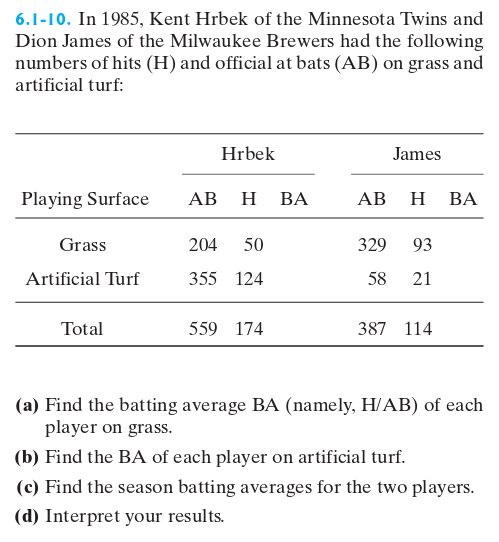
\includegraphics{images/num2.png} 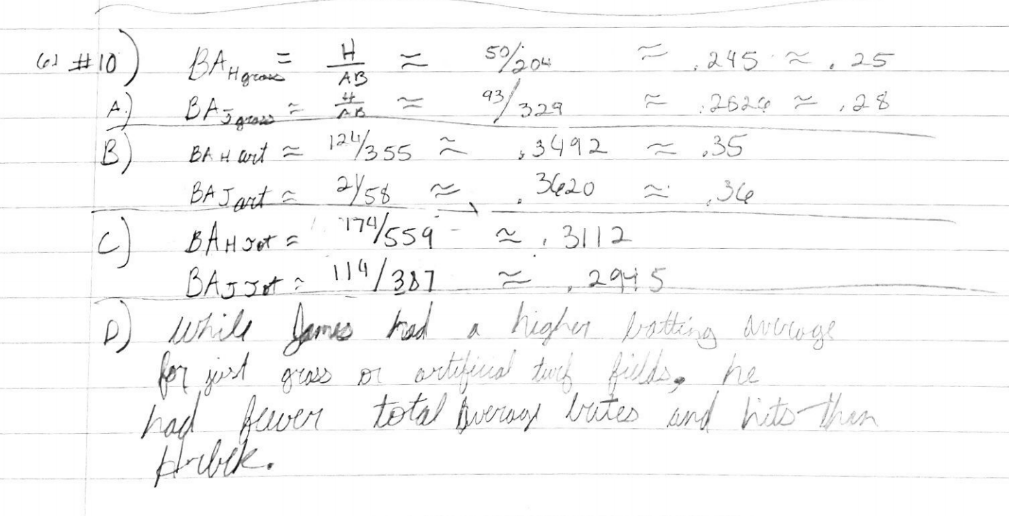
\includegraphics{images/solution2.png}

    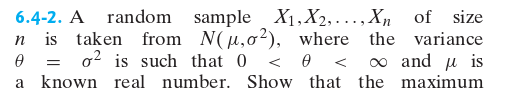
\includegraphics{images/num3.1.png} 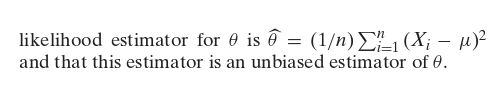
\includegraphics{images/num3.2.png}

    \begin{figure}
\centering
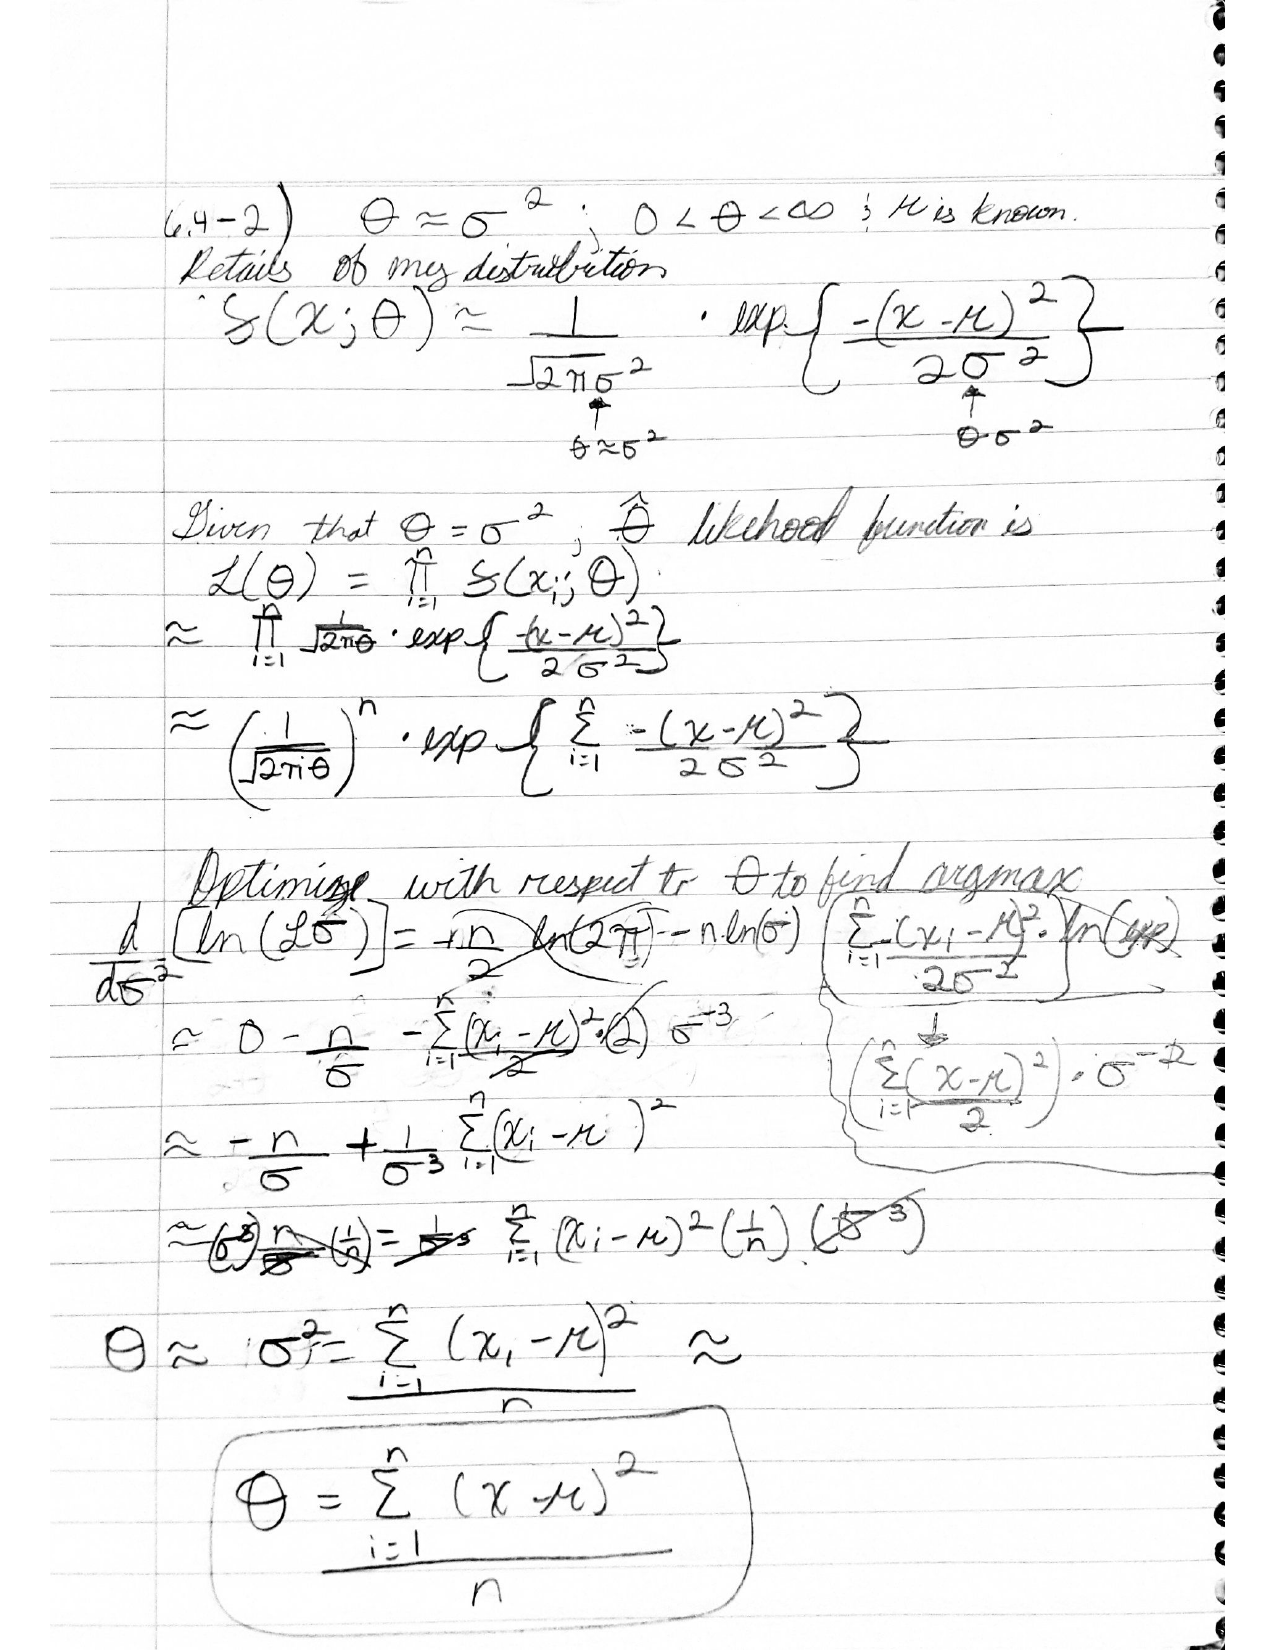
\includegraphics{images/solution3.png}
\caption{alt text}
\end{figure}

    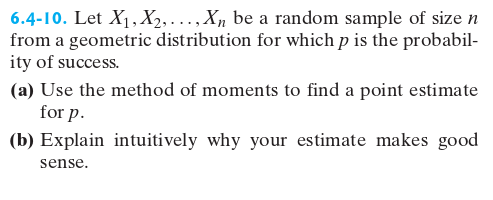
\includegraphics{images/num4.1.png} 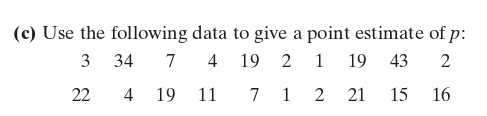
\includegraphics{images/num4.2.png}

    \hypertarget{a}{%
\subsection{A)}\label{a}}

    \begin{figure}
\centering
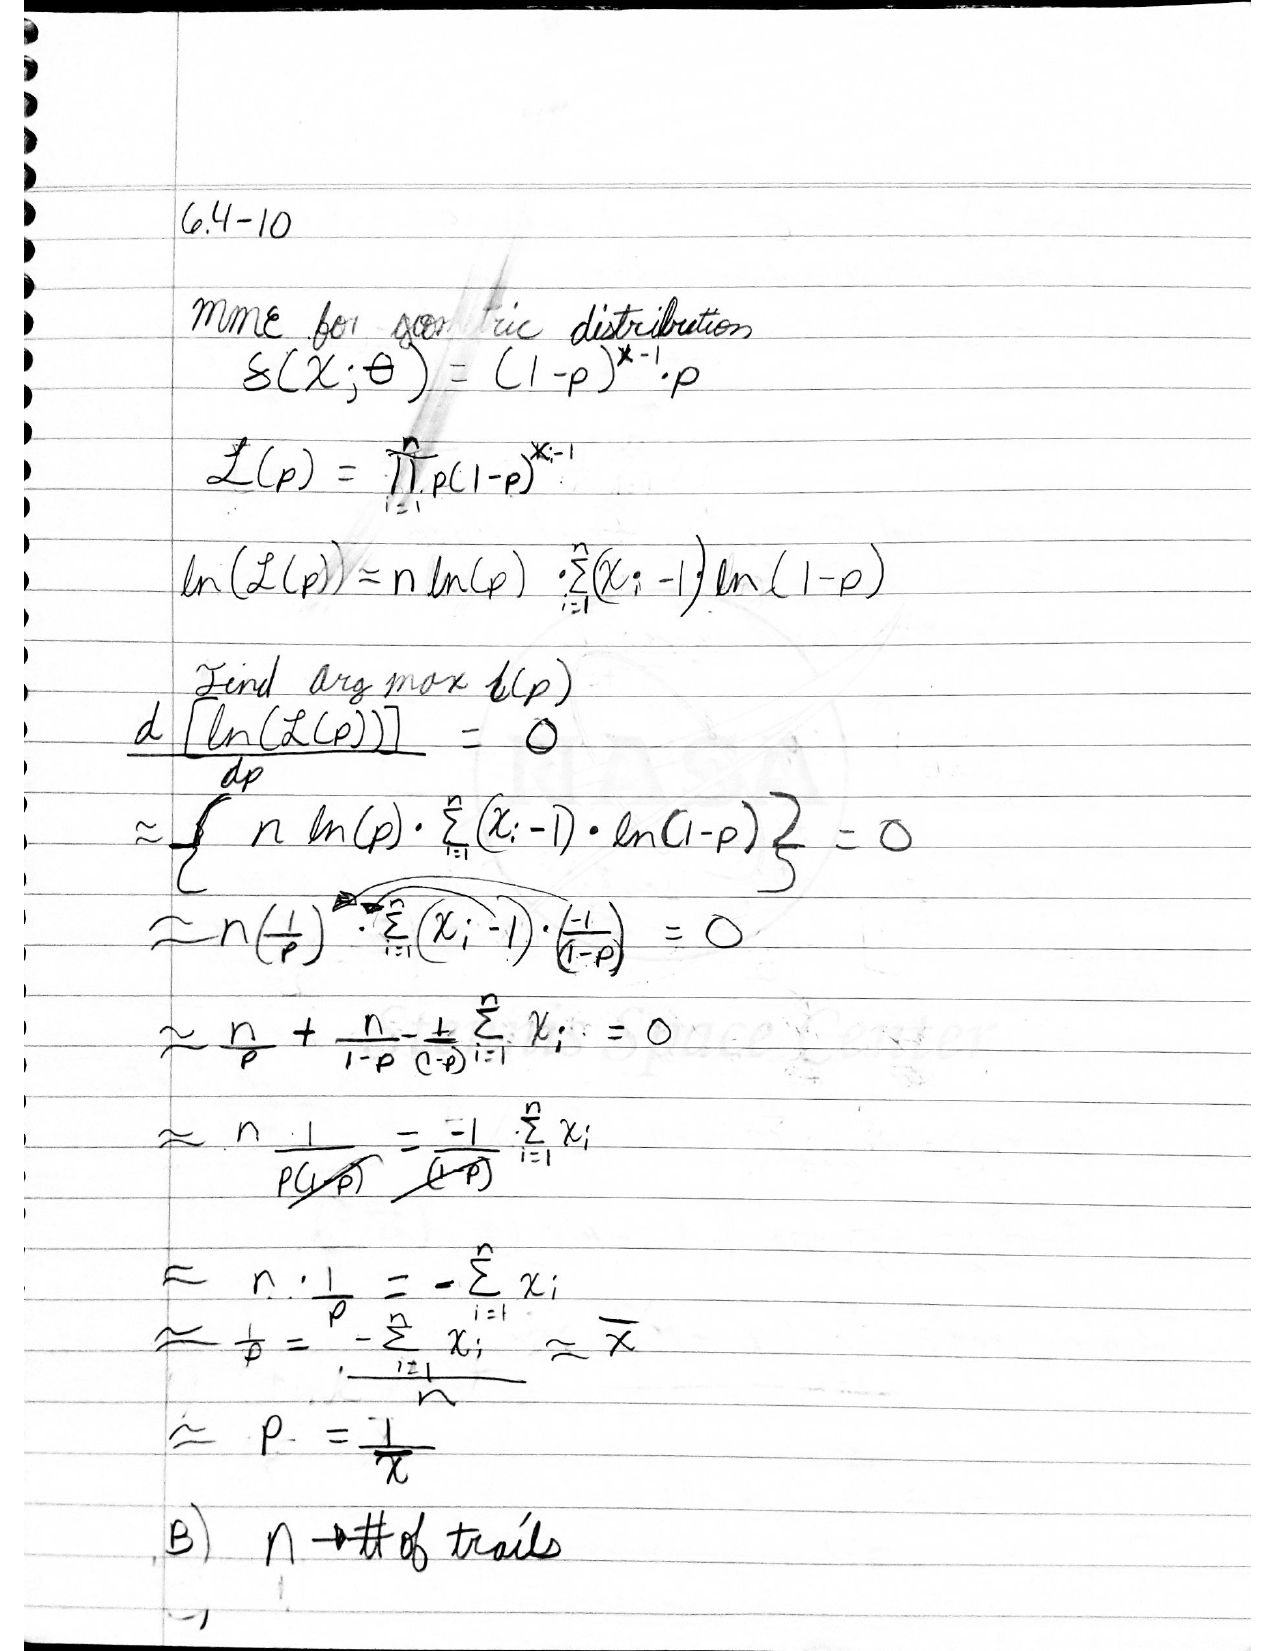
\includegraphics{images/solution4.png}
\caption{alt text}
\end{figure}

    \[\hat{p}^{ML}=\frac{n}{\left(\sum_{i=1}^{n}{X}_{i} \right)} = \frac{1}{\frac{\left(\sum_{i=1}^{n}{X}_{i} \right)}{n}} =\frac{1}{\mathbb{E}(X_i)} =\frac{1}{\bar{X}}\]

    \hypertarget{b}{%
\subsection{B)}\label{b}}

\hypertarget{the-geometric-distribution-characterizes-n-independent-trails-until-the-first-success.-1-pk-1p}{%
\subsubsection{\texorpdfstring{The geometric distribution characterizes
n independent trails until the first success.
\((1-p)^{K-1}*p\)}{The geometric distribution characterizes n independent trails until the first success. (1-p)\^{}\{K-1\}*p}}\label{the-geometric-distribution-characterizes-n-independent-trails-until-the-first-success.-1-pk-1p}}

\hypertarget{being-that-we-have-n-trails-and-the-probility-of-each-trail-success-before-we-reach-our-first-success-is-defined-as-1-pk-1}{%
\subsubsection{\texorpdfstring{Being that we have \(n\) trails and the
probility of each trail success before we reach our first success is
defined as \((1-p)^{K-1}\)
\ldots{}}{Being that we have n trails and the probility of each trail success before we reach our first success is defined as (1-p)\^{}\{K-1\} \ldots{}}}\label{being-that-we-have-n-trails-and-the-probility-of-each-trail-success-before-we-reach-our-first-success-is-defined-as-1-pk-1}}

\hypertarget{we-can-deduce-that-the-probability-of-each-trail-being-a-success-n-p-barx}{%
\subsubsection{\texorpdfstring{We can deduce that the probability of
each trail being a success
\(n * p = \bar{X}\)}{We can deduce that the probability of each trail being a success n * p = \textbackslash{}bar\{X\}}}\label{we-can-deduce-that-the-probability-of-each-trail-being-a-success-n-p-barx}}

\hypertarget{but-given-only-the-nth-trail-can-be-a-success-the-probability-of-the-first-momentexpected-value}{%
\subsubsection{\texorpdfstring{But given only the \(nth\) trail can be a
success the probability of the first moment(expected
value)}{But given only the nth trail can be a success the probability of the first moment(expected value)}}\label{but-given-only-the-nth-trail-can-be-a-success-the-probability-of-the-first-momentexpected-value}}

\hypertarget{approx-p-frac1barx}{%
\subsection{\texorpdfstring{\(\approx p = \frac{1}{\bar{X}}\)}{\textbackslash{}approx p = \textbackslash{}frac\{1\}\{\textbackslash{}bar\{X\}\}}}\label{approx-p-frac1barx}}

    \hypertarget{c-method-of-moments-estimation-at-p-0.07936507936507936}{%
\subsection{C) Method of Moments estimation at p:
0.07936507936507936}\label{c-method-of-moments-estimation-at-p-0.07936507936507936}}

    \begin{Verbatim}[commandchars=\\\{\}]
{\color{incolor}In [{\color{incolor}2}]:} \PY{n}{data} \PY{o}{=} \PY{n}{load\PYZus{}sample\PYZus{}data}\PY{p}{(}\PY{l+m+mi}{6}\PY{p}{,}\PY{l+m+mi}{4}\PY{p}{,}\PY{l+m+mi}{10}\PY{p}{,} \PY{n}{display}\PY{o}{=}\PY{k+kc}{True}\PY{p}{)}
        \PY{n+nb}{print}\PY{p}{(}\PY{n}{f}\PY{l+s+s2}{\PYZdq{}}\PY{l+s+s2}{Method of Moments estimation at p: }\PY{l+s+s2}{\PYZob{}}\PY{l+s+s2}{mme\PYZus{}geo(data)\PYZcb{}}\PY{l+s+s2}{\PYZdq{}}\PY{p}{)}
\end{Verbatim}


    \begin{Verbatim}[commandchars=\\\{\}]
Loaded E6\_4-10.txt sucessfully.
[ 3 34  7  4 19  2  1 19 43  2 22  4 19 11  7  1  2 21 15 16]
Method of Moments estimation at p: 0.07936507936507936

    \end{Verbatim}

    \begin{figure}
\centering
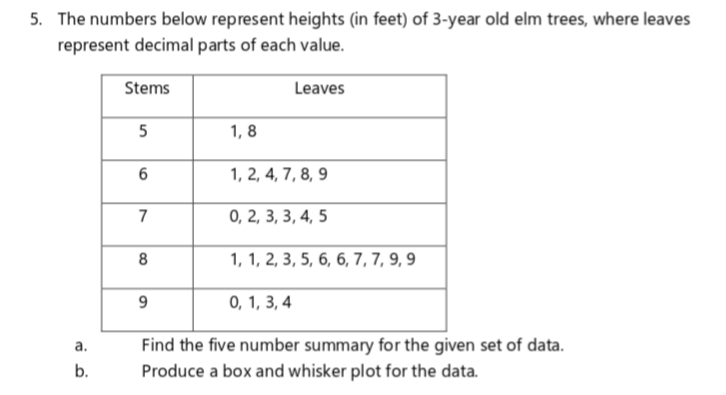
\includegraphics{images/num5.png}
\caption{alt text}
\end{figure}

    \begin{Verbatim}[commandchars=\\\{\}]
{\color{incolor}In [{\color{incolor}3}]:} \PY{c+c1}{\PYZsh{} Find the Five Num Summary of the data}
        \PY{n}{sl\PYZus{}plot} \PY{o}{=} \PY{n}{np}\PY{o}{.}\PY{n}{array}\PY{p}{(}\PY{p}{[}\PY{l+m+mi}{51}\PY{p}{,}\PY{l+m+mi}{58}\PY{p}{,}\PY{l+m+mi}{61}\PY{p}{,}\PY{l+m+mi}{62}\PY{p}{,}\PY{l+m+mi}{64}\PY{p}{,} \PY{l+m+mi}{67}\PY{p}{,}\PY{l+m+mi}{68}\PY{p}{,}\PY{l+m+mi}{69}\PY{p}{,} \PY{l+m+mi}{70}\PY{p}{,} \PY{l+m+mi}{72}\PY{p}{,}  \PY{l+m+mi}{73}\PY{p}{,} \PY{l+m+mi}{73}\PY{p}{,} \PY{l+m+mi}{74}\PY{p}{,} \PY{l+m+mi}{75}\PY{p}{,} \PY{l+m+mi}{81}\PY{p}{,} \PY{l+m+mi}{81}\PY{p}{,} \PY{l+m+mi}{82}\PY{p}{,} \PY{l+m+mi}{83}\PY{p}{,} \PY{l+m+mi}{85}\PY{p}{,} \PY{l+m+mi}{86}\PY{p}{,} \PY{l+m+mi}{86}\PY{p}{,} \PY{l+m+mi}{87}\PY{p}{,} \PY{l+m+mi}{87}\PY{p}{,} \PY{l+m+mi}{89}\PY{p}{,} \PY{l+m+mi}{89}\PY{p}{,} \PY{l+m+mi}{90}\PY{p}{,} \PY{l+m+mi}{91}\PY{p}{,} \PY{l+m+mi}{93}\PY{p}{,} \PY{l+m+mi}{94}\PY{p}{]}\PY{p}{)}
        \PY{n}{minn} \PY{o}{=} \PY{n}{np}\PY{o}{.}\PY{n}{min}\PY{p}{(}\PY{n}{sl\PYZus{}plot}\PY{p}{)}
        \PY{n}{median} \PY{o}{=} \PY{n}{np}\PY{o}{.}\PY{n}{median}\PY{p}{(}\PY{n}{sl\PYZus{}plot}\PY{p}{)}
        \PY{n}{mx} \PY{o}{=} \PY{n}{np}\PY{o}{.}\PY{n}{max}\PY{p}{(}\PY{n}{sl\PYZus{}plot}\PY{p}{)}
        \PY{n}{qr1} \PY{o}{=} \PY{n}{np}\PY{o}{.}\PY{n}{median}\PY{p}{(}\PY{n}{sl\PYZus{}plot}\PY{p}{[}\PY{p}{:}\PY{l+m+mi}{13}\PY{p}{]}\PY{p}{)}
        \PY{n}{qr3} \PY{o}{=} \PY{n}{np}\PY{o}{.}\PY{n}{median}\PY{p}{(}\PY{n}{sl\PYZus{}plot}\PY{p}{[}\PY{l+m+mi}{15}\PY{p}{:}\PY{p}{]}\PY{p}{)}
        
        \PY{n+nb}{print}\PY{p}{(}\PY{l+s+s2}{\PYZdq{}}\PY{l+s+s2}{Five Number Summary}\PY{l+s+s2}{\PYZdq{}}\PY{p}{)}
        \PY{n+nb}{print}\PY{p}{(}\PY{l+s+s2}{\PYZdq{}}\PY{l+s+s2}{=}\PY{l+s+s2}{\PYZdq{}}\PY{o}{*}\PY{l+m+mi}{20}\PY{p}{)}
        \PY{n+nb}{print}\PY{p}{(}\PY{n}{f}\PY{l+s+s2}{\PYZdq{}}\PY{l+s+s2}{Min: }\PY{l+s+si}{\PYZob{}minn\PYZcb{}}\PY{l+s+s2}{, First Quartile: }\PY{l+s+si}{\PYZob{}qr1\PYZcb{}}\PY{l+s+s2}{, Median: }\PY{l+s+si}{\PYZob{}median\PYZcb{}}\PY{l+s+s2}{, Third Quartile: }\PY{l+s+si}{\PYZob{}qr3\PYZcb{}}\PY{l+s+s2}{, Maximum: }\PY{l+s+si}{\PYZob{}mx\PYZcb{}}\PY{l+s+s2}{\PYZdq{}}\PY{p}{)}
        
        \PY{c+c1}{\PYZsh{} Plot and Display Box and whisker plot}
        \PY{n}{sns}\PY{o}{.}\PY{n}{set}\PY{p}{(}\PY{n}{style}\PY{o}{=}\PY{l+s+s2}{\PYZdq{}}\PY{l+s+s2}{whitegrid}\PY{l+s+s2}{\PYZdq{}}\PY{p}{)}
        \PY{n}{ax} \PY{o}{=} \PY{n}{sns}\PY{o}{.}\PY{n}{boxplot}\PY{p}{(}\PY{n}{x}\PY{o}{=}\PY{n}{sl\PYZus{}plot}\PY{p}{)}
        \PY{n}{ax}\PY{o}{.}\PY{n}{set}\PY{p}{(}\PY{n}{xlabel}\PY{o}{=}\PY{l+s+s1}{\PYZsq{}}\PY{l+s+s1}{Height of Elm Trees After 3 years}\PY{l+s+s1}{\PYZsq{}}\PY{p}{)}
        \PY{n}{plt}\PY{o}{.}\PY{n}{show}\PY{p}{(}\PY{p}{)}
\end{Verbatim}


    \begin{Verbatim}[commandchars=\\\{\}]
Five Number Summary
====================
Min: 51, First Quartile: 68.0, Median: 81.0, Third Quartile: 87.0, Maximum: 94

    \end{Verbatim}

    \begin{center}
    \adjustimage{max size={0.9\linewidth}{0.9\paperheight}}{output_17_1.png}
    \end{center}
    { \hspace*{\fill} \\}
    
    \begin{figure}
\centering
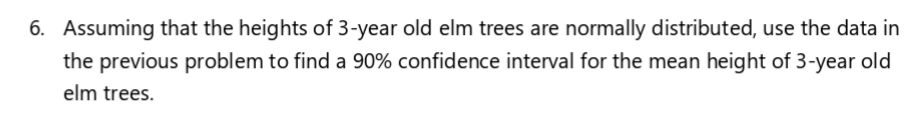
\includegraphics{images/num6.png}
\caption{alt text}
\end{figure}

    \hypertarget{find-the-90-confidence-interval-using-the-z-distribution}{%
\subsection{Find the 90\% Confidence interval using the Z
distribution?}\label{find-the-90-confidence-interval-using-the-z-distribution}}

    \begin{Verbatim}[commandchars=\\\{\}]
{\color{incolor}In [{\color{incolor}48}]:} \PY{n}{mean} \PY{o}{=} \PY{n}{sample\PYZus{}mean}\PY{p}{(}\PY{n}{sl\PYZus{}plot}\PY{p}{)}
         \PY{n}{var} \PY{o}{=} \PY{n}{sample\PYZus{}variance}\PY{p}{(}\PY{n}{sl\PYZus{}plot}\PY{p}{)}
         \PY{n}{std} \PY{o}{=} \PY{n}{var} \PY{o}{*}\PY{o}{*}\PY{o}{.}\PY{l+m+mi}{5}
         \PY{n}{n} \PY{o}{=} \PY{n+nb}{len}\PY{p}{(}\PY{n}{sl\PYZus{}plot}\PY{p}{)}
         
         \PY{c+c1}{\PYZsh{}\PYZsh{} Look up this value on table}
         \PY{n}{z\PYZus{}area} \PY{o}{=} \PY{l+m+mi}{1} \PY{o}{\PYZhy{}} \PY{p}{(}\PY{p}{(}\PY{l+m+mi}{1} \PY{o}{\PYZhy{}} \PY{o}{.}\PY{l+m+mi}{90}\PY{p}{)}\PY{o}{/} \PY{l+m+mi}{2}\PY{p}{)}
         \PY{n}{z\PYZus{}score} \PY{o}{=} \PY{l+m+mf}{1.65}
         \PY{n}{interval} \PY{o}{=} \PY{n}{z\PYZus{}score} \PY{o}{*} \PY{p}{(}\PY{n}{std} \PY{o}{/} \PY{p}{(}\PY{n}{n} \PY{o}{*}\PY{o}{*} \PY{o}{.}\PY{l+m+mi}{5}\PY{p}{)}\PY{p}{)}
         
         \PY{n}{conf\PYZus{}interval} \PY{o}{=} \PY{n}{np}\PY{o}{.}\PY{n}{array}\PY{p}{(}\PY{p}{[}\PY{n}{mean} \PY{o}{\PYZhy{}} \PY{n}{interval}\PY{p}{,} \PY{n}{mean} \PY{o}{+} \PY{n}{interval}\PY{p}{]}\PY{p}{)}
         \PY{n+nb}{print}\PY{p}{(}\PY{n}{conf\PYZus{}interval}\PY{p}{)}
\end{Verbatim}


    \begin{Verbatim}[commandchars=\\\{\}]
[73.7225434  80.82918074]

    \end{Verbatim}

    \hypertarget{x-z}{%
\section{\texorpdfstring{\$ \bar\{X\} \pm Z * \frac{ \sigma} {\sqrt{n}}
\$}{\$ \{X\} Z *  \$}}\label{x-z}}

\hypertarget{lower-bound-73.7225434}{%
\section{Lower bound: 73.7225434}\label{lower-bound-73.7225434}}

\hypertarget{upper-bound-80.82918074}{%
\section{Upper bound: 80.82918074}\label{upper-bound-80.82918074}}


    % Add a bibliography block to the postdoc
    
    
    
    \end{document}
